\documentclass{beamer}

%\usepackage{csvsimple-l3}
\usepackage{booktabs}
\usepackage{multirow}
%\usepackage{graphicx}
%\usepackage{biblatex}
\usepackage{listings}
\usepackage{siunitx}
\usepackage{pgfplots}
\usepackage{tikz-cd}
\usepackage{subcaption}
%\usepackage{comment}
%\usepackage{hyperref}
\usepackage{ulem}
\usepackage{multicol}
\usepackage[nolinks]{qrcode}

\pgfplotsset{compat=1.18}
\tikzset{ dots/.style = {mark=*, draw=black, mark size=.5pt} }
\usetikzlibrary{external}
%\usetikzlibrary{matrix}
%\tikzexternalize
%\addbibresource{bracket.bib}

\title{Seeding Statistics of Elimination Tournaments}
\author{Timothy Prescott}
\date{\today}

\begin{document}

\begin{frame}
\maketitle
\end{frame}

\begin{frame}
\frametitle{Alternative Titles}
\begin{center}\Large\color{blue}
\sout{Statistics of Seeding of Tournaments of Elimination}\\
\sout{Statistics of Seeding of Elimination Tournaments}\\
Seeding Statistics of Elimination Tournaments\\
\sout{Elimination Tournaments' Seeding Statistics}
\end{center}
\end{frame}

\begin{frame}
\frametitle{Exploring Alternative Titles}\centering
\begin{tikzcd}[tips=false, column sep=1em, row sep=1.5em, ampersand replacement=\&]
\& \text{St of Se of To of El} \ar{dl}\ar{d}\ar{dr}\\
\text{St of Se of El To} \ar{d} \ar{dr} \& \text{To of El St of Se} \ar{dl} \ar{dr} \& \text{Se St of To of El} \ar{dl} \ar{d} \\
\text{El To St of Se} \& \text{Se St of El To} \& \text{To of El Se St} \\
\& \text{El To Se St} \ar{ul} \ar{u} \ar{ur}
\end{tikzcd}
\end{frame}

\begin{frame}
\frametitle{Wikipedia}
March Madness\\
Wikipedia:\\
``[Year] NCAA Division I $\underbrace{\text{[men's/women's]}}_{\text{after 1981}}$ basketball tournament'':
\end{frame}

\begin{frame}
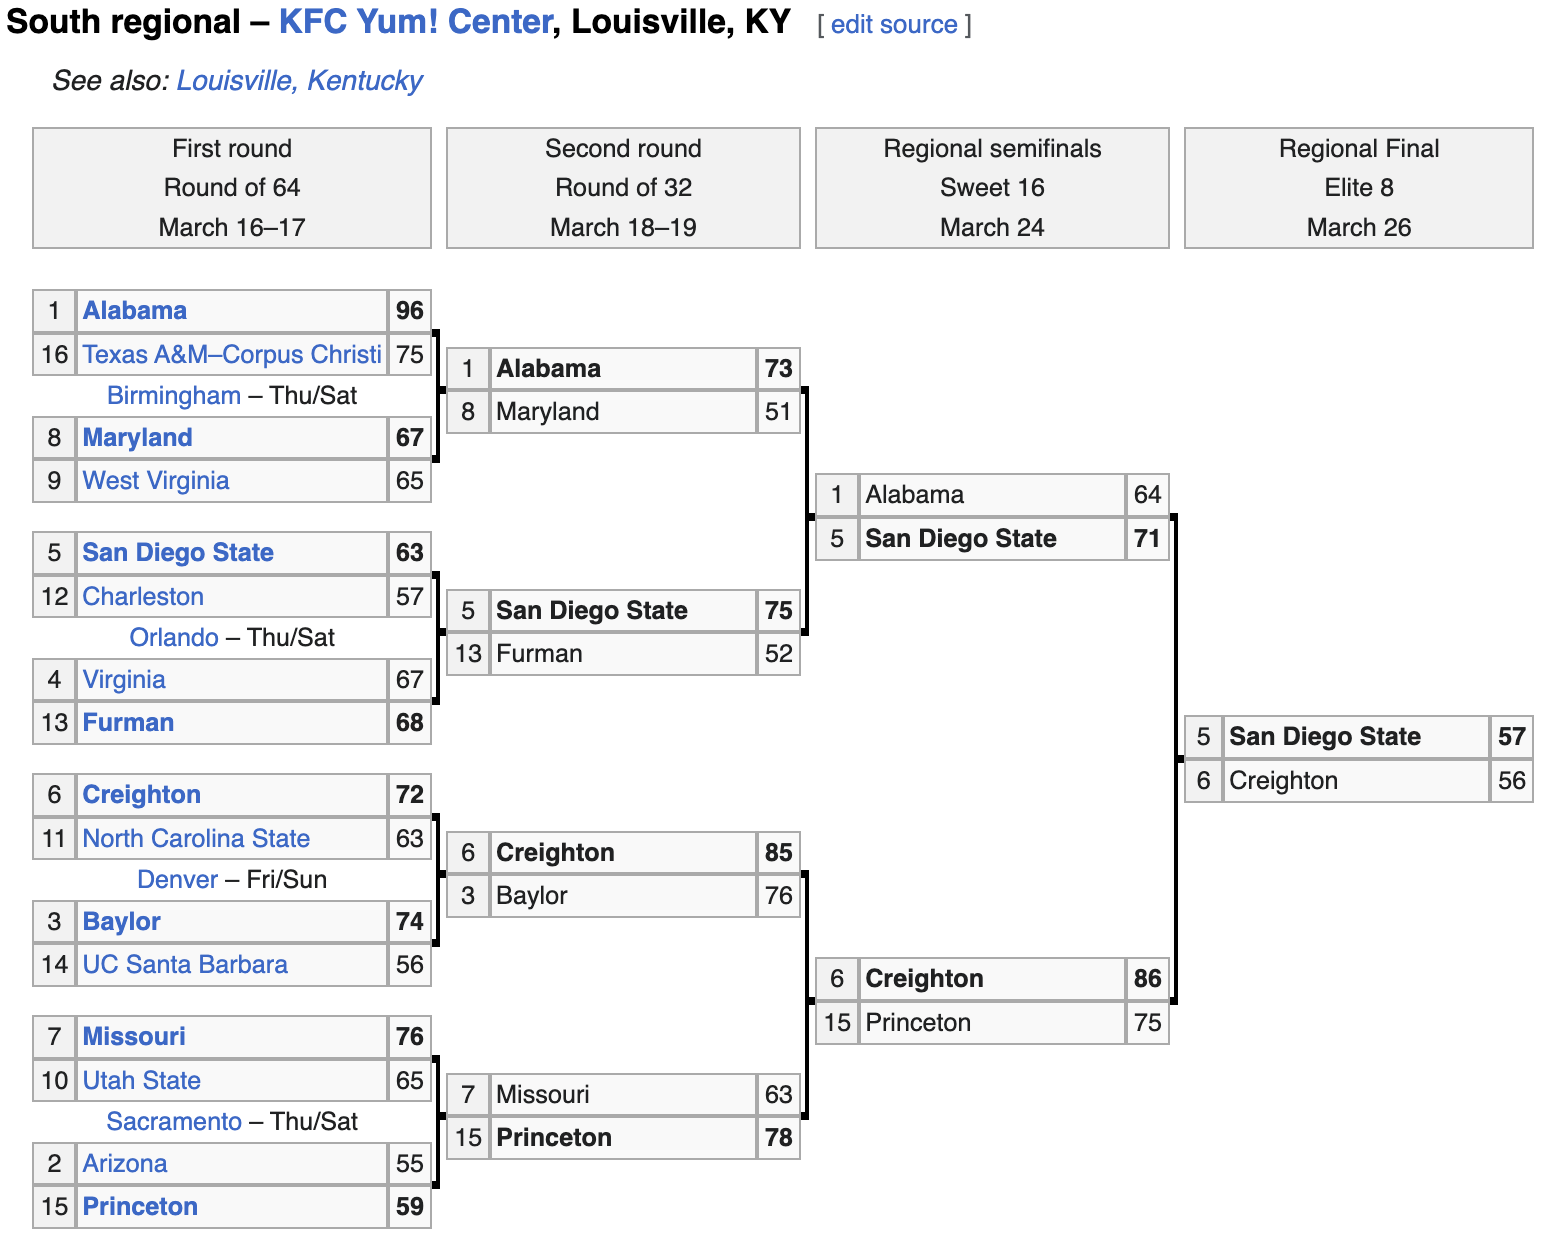
\includegraphics[width=\linewidth]{../paper/2023bracket}
\end{frame}

\begin{frame}[fragile]
%The source for this bracket is
\begin{lstlisting}[basicstyle=\tiny,breaklines=true]
...
| RD1-seed01=1
| RD1-team01= '''[[2022-23 Alabama Crimson Tide men's basketball team|Alabama]]'''
| RD1-score01='''96'''
| RD1-seed02=16
| RD1-team02= [[2022-23 Texas A&M-Corpus Christi Islanders men's basketball team|Texas A&M-Corpus Christi]]
| RD1-score02=75
 
| RD1-seed03=8
| RD1-team03= '''[[2022-23 Maryland Terrapins men's basketball team|Maryland]]'''
| RD1-score03='''67'''
| RD1-seed04=9
| RD1-team04= [[2022-23 West Virginia Mountaineers men's basketball team|West Virginia]]
| RD1-score04=65
 
| RD1-seed05=5
| RD1-team05= '''[[2022-23 San Diego State Aztecs men's basketball team|San Diego State]]'''
| RD1-score05='''63'''
| RD1-seed06=12
| RD1-team06= [[2022-23 College of Charleston Cougars men's basketball team|Charleston]]
| RD1-score06=57
 
| RD1-seed07=4
| RD1-team07=[[2022-23 Virginia Cavaliers men's basketball team|Virginia]]
| RD1-score07=67
| RD1-seed08= 13
| RD1-team08= '''[[2022-23 Furman Paladins men's basketball team|Furman]]'''
| RD1-score08='''68'''
...
\end{lstlisting}
\end{frame}

\begin{frame}
\setlength{\tabcolsep}{0px}
\tiny
\frametitle{Winning fractions (men's)}
\noindent
\begin{tabular*}{\textwidth}{ @{\extracolsep{\fill}} r *{16}{S[table-format=1.2, table-auto-round]} }\toprule
\input{../bbm/D1/winlossprobs}
\end{tabular*}
\normalsize
Amount of time that seed [row] defeats seed [column], $n=2582$.
\end{frame}

\begin{frame}
\setlength{\tabcolsep}{0px}
\tiny
\frametitle{Winning fractions (women's)}
\begin{tabular*}{\textwidth}{ @{\extracolsep{\fill}} r *{16}{S[table-format=1.2, table-auto-round]} }\toprule
\input{../bbw/D1/winlossprobs}
\end{tabular*}
\normalsize
Amount of time that seed [row] defeats seed [column], $n=1843$.
\end{frame}

\begin{frame}
\frametitle{Seed differential v fraction won by favored}
%\begin{minipage}{.48\textwidth}\centering
\begin{tikzpicture}
\begin{axis}[width=.48\linewidth-30pt,height=.48\linewidth,xmin=0,xmax=15.1,ymin=0,ymax=1,scale only axis,
axis y line=left,y axis line style=-,ticklabel style={font=\small}]
\addplot[dots](0,.5);
\addplot[domain=0:15]{1/(1+exp(-.161*x))};
% analyze.analyze_winloss('bbm/D1/winloss.csv')
\input{../bbm/D1/winlossplot}
\end{axis}
\end{tikzpicture}%\\
%Men's. $\beta=0.161$
%\end{minipage}%
\hfill
%\begin{minipage}{.48\textwidth}\centering
\begin{tikzpicture}
\begin{axis}[width=.48\linewidth-30pt,height=.48\linewidth,xmin=0,xmax=15.1,ymin=0,ymax=1,scale only axis,
axis y line=left,y axis line style=-,ticklabel style={font=\small}]
\addplot[dots](0,.5);
\addplot[domain=0:15]{1/(1+exp(-.276*x))};
% analyze.analyze_winloss('bbw/D1/winloss.csv')
\input{../bbw/D1/winlossplot}
\end{axis}
\end{tikzpicture}%\\
%Women's. $\beta=0.276$
%\end{minipage}
\\\medskip
\hfill Men's. $\beta=0.161$\hfill Women's. $\beta=0.276$\hfill\null\\
Logistic best fit: $(1+\exp\{-\beta(x-\mu)\})^{-1}$, but $\mu=0$ by symmetry.\\
Upsets with seed differential 7 or higher are significantly more likely ($p=\num{3.8e-12}$) in the men's tournament (18\%) than the women's (8\%).
\end{frame}

\begin{frame}
\frametitle{After an upset}
Fraction of time that the better seeded team wins in the second round, after one first round upset.  (Minimum 10 games.)
\begin{center}
\begin{tabular}{ c *2{S[table-format=2(2), separate-uncertainty]} }\toprule
Seeds & {Men's (\%)} & {Women's (\%)} \\\midrule
1 v \phantom19 & 89(6) & 93(5) \\
2 v 10 & 62(12) & 84(9) \\
3 v 11 & 66(12) & 68(13) \\
4 v 12 & 69(13) & 82(13) \\
5 v 13 & 79(15) \\
6 v 14 & 80(16) \\\addlinespace
overall & 75(5) & 84(5)\\
prediction & 78.4 & 90.1 \\\bottomrule
\end{tabular}
\end{center}
An upset may lead to another upset, but not significantly so.
\end{frame}

\begin{frame}
\frametitle{Play-in winners}
Number of games won in first round in the men's tournament, by seed, where the worse seed was (not) the winner of a play-in game.  Also significance of the statement ``Play-in winners are more likely to have an upset in their first round.''
\begin{center}
\begin{tabular}{ c *{10}{S[table-format=2]} }\toprule
Seed & {6} & 11 & {5} & 12 & {4} & 13 & {3} & 14 & {1} & 16 \\\cmidrule(r){2-3}\cmidrule(lr){4-5}\cmidrule(lr){6-7}\cmidrule(lr){8-9}\cmidrule(l){10-11}
Play-in & 9 & 9 & 3 & 1 & 0 & 1 & 1 & 0 & 33 & 1 \\
Non-play-in & 40 & 30 & 50 & 34 & 68 & 19 & 78 & 19 & 53 & 1 \\\addlinespace
% eg, scipy.stats.fisher_exact([[9,9],[40,30]],'less'), etc.
$p$ & \multicolumn2c{0.39} & \multicolumn2c{0.87} & \multicolumn2c{0.23} & \multicolumn2c{1} & \multicolumn2c{0.63}
\\\bottomrule
\end{tabular}
\end{center}
$p$ values much too high to make any conclusions.
\end{frame}

\begin{frame}
\frametitle{Team names problem \#1: Southern Connecticut}
\begin{multicols}{2}
\begin{enumerate}
\item S. Conn. State
\item S. Connecticut
\item S. Connecticut State
\item So. Conn. State
\item So. Connecticut St
\item So. Connecticut St.
\item So. Connecticut
\item South Connecticut St.
\item Southern Conn.
\item Southern Conn. St.
\item Southern Connecticut
\item Southern Connecticut State
\end{enumerate}
\end{multicols}
Solution: expand (almost) all abbreviations.  Drop unnecessary words.
\end{frame}

\begin{frame}
\frametitle{Team names problem \#2: USC}
\begin{center}
\begin{tabular}{c @{\qquad} c}\toprule
Southern California & South Carolina \\\midrule
Trojans & Gamecocks \\
Southern Cal & South Car \\
Pac(ific)?-(8$|$10$|$12) Conference \\\bottomrule
\end{tabular}
\end{center}
Also: USC Aiken, USC Spartanburg, USC Upstate.\\\bigskip
Also also: Saint John's, Notre Dame, Miami, and many many many more.
\end{frame}

\begin{frame}
\frametitle{Team names problem \#3: Misspellings}
\begin{multicols}{2}
\begin{itemize}
\item IIllinois
\item Florida Gulf Goast
\item Case \underline{Western}
\item Saint Benedict\sout{'s} (MN)
\item St. Benedict\underline{'s} (KS)
\item Up\sout psala
\item College \underline{of} Charleston
\item McMurr\sout ay
\item Rensse\sout al\underline aer
\item Washingt\sout non
\item S\underline tate
\item Manka\sout ato
\item Baker\underline sfield
\item Mont\sout egomery
\item Montgome\underline ry
\item De\sout s\underline Sales
\end{itemize}
\end{multicols}
And many many many more.
\end{frame}

\begin{frame}
\frametitle{Looking at a single team's seed differential v fraction won}
\begin{minipage}{.48\textwidth}
\begin{tikzpicture}
\begin{axis}[width=\linewidth-3pt,height=\linewidth,xmin=-16,xmax=16,ymin=0,ymax=1,axis y line=center,scale only axis,
y axis line style=-,x axis line style=<->,clip=false,xtick={-10,10},ticklabel style={font=\footnotesize},tickwidth=.3cm]
% analyze.get_team_performance('bbm', 'D1', 'North Carolina')
\addplot[domain=-15:15]{1/(1+exp(-.192*(x+2.78)))};
\addplot[dots](-2.78,.5)node[left]{\tiny$\mu=-2.78$};
\addplot[dots](8,1)node[above]{\tiny11};
\addplot[dots](3,1)node[below]{\tiny7};
\addplot[dots](2,1)node[above]{\tiny4};
\addplot[dots](5,1)node[below]{\tiny11};
\addplot[dots](0,1)node[above]{\tiny4};
\addplot[dots](1,1)node[below]{\tiny14};
\addplot[dots](7,1)node[below]{\tiny7};
\addplot[dots](13,1)node[below]{\tiny7};
\addplot[dots](9,1)node[below]{\tiny6};
\addplot[dots](11,1)node[below]{\tiny3};
\addplot[dots](15,1)node[below]{\tiny14};
\addplot[dots](4,1)node[above]{\tiny7};
\addplot[dots](-7,1)node[below]{\tiny3};
\addplot[dots](-1,1)node[below]{\tiny2};
\addplot[dots](-4,1)node[above]{\tiny2};
\addplot[dots](12,1)node[above]{\tiny1};
\addplot[dots](-6,1)node[above]{\tiny1};
\addplot[dots](2,0)node[below]{\tiny4};
\addplot[dots](3,0)node[above]{\tiny2};
\addplot[dots](6,0)node[below]{\tiny1};
\addplot[dots](-1,0)node[above]{\tiny2};
\addplot[dots](1,0)node[above]{\tiny6};
\addplot[dots](-4,0)node[below]{\tiny1};
\addplot[dots](-3,0)node[above]{\tiny6};
\addplot[dots](8,0)node[below]{\tiny2};
\addplot[dots](0,0)node[below]{\tiny2};
\addplot[dots](11,0)node[above]{\tiny1};
\addplot[dots](5,0)node[above]{\tiny2};
\addplot[dots](-7,0)node[above]{\tiny2};
\addplot[dots](4,0)node[below]{\tiny1};
\end{axis}
\end{tikzpicture}\\
%\parbox{\textwidth}{\centering
North Carolina men.\\
$N=136$, $\beta=0.192$.%}
\end{minipage}%
\hfill
\begin{minipage}{.48\textwidth}
\begin{tikzpicture}
\begin{axis}[width=\linewidth-3pt,height=\linewidth,xmin=-16,xmax=16,ymin=0,ymax=1,axis y line=center,scale only axis,
y axis line style=-,x axis line style=<->,clip=false,xtick={-10,10},ticklabel style={font=\footnotesize},tickwidth=.3cm]
% analyze.get_team_performance('bbw', 'D1', 'Tennessee')
\addplot[domain=-15:15]{1/(1+exp(-.304*(x+1.92)))};
\addplot[dots](-1.92,.5)node[left]{\tiny$\mu=-1.92$};
\addplot[dots](5,1)node[below]{\tiny6};
\addplot[dots](1,1)node[below]{\tiny13};
\addplot[dots](-1,1)node[below]{\tiny7};
\addplot[dots](7,1)node[below]{\tiny14};
\addplot[dots](3,1)node[below]{\tiny18};
\addplot[dots](-2,1)node[above]{\tiny4};
\addplot[dots](0,1)node[above]{\tiny10};
\addplot[dots](-3,1)node[below]{\tiny1};
\addplot[dots](8,1)node[above]{\tiny14};
\addplot[dots](4,1)node[above]{\tiny4};
\addplot[dots](2,1)node[above]{\tiny6};
\addplot[dots](15,1)node[below]{\tiny15};
\addplot[dots](11,1)node[below]{\tiny3};
\addplot[dots](13,1)node[below]{\tiny5};
\addplot[dots](9,1)node[below]{\tiny5};
\addplot[dots](12,1)node[above]{\tiny1};
\addplot[dots](6,1)node[above]{\tiny1};
\addplot[dots](-5,1)node[below]{\tiny1};
\addplot[dots](-4,1)node[above]{\tiny1};
\addplot[dots](-1,0)node[above]{\tiny7};
\addplot[dots](3,0)node[above]{\tiny9};
\addplot[dots](1,0)node[above]{\tiny6};
\addplot[dots](-2,0)node[below]{\tiny1};
\addplot[dots](-3,0)node[above]{\tiny4};
\addplot[dots](0,0)node[below]{\tiny4};
\addplot[dots](2,0)node[below]{\tiny1};
\addplot[dots](7,0)node[above]{\tiny1};
\addplot[dots](-5,0)node[above]{\tiny1};
\end{axis}
\end{tikzpicture}\\
Tennessee women.\\
$N=163$, $\beta=0.304$
\end{minipage}
\end{frame}

\begin{frame}
\frametitle{\# Games v expected reseeding}
\begin{minipage}{.48\textwidth}
\begin{tikzpicture}
\begin{axis}[width=.98\linewidth,height=.8\linewidth,axis y line=left,axis x line=center,y axis line style=<->,
	xmin=9.1,xmax=170,ymin=-10,ymax=10,xmode=log,xtick={10,20,50,100},xticklabels={10,20,50,100},xlabel={\# Games},ylabel={Expected reseeding},
	ticklabel style={font=\small},tickwidth=.3cm,xlabel style={yshift=-7ex},restrict y to domain=-10:10]
 \addplot[dots] table[col sep=comma,x=Games,y=Reseed,only marks]{../bbm/D1/reseed.csv};
% \csvreader[head to column names, filter fp = {\Games>9 && \Rate>0.01}]
%   {../bbm/D1/reseed.csv}{}{\addplot[dots](\Games,\Reseed);}
\end{axis}
\end{tikzpicture}\\
Men's
\end{minipage}%
\hfill
\begin{minipage}{.48\textwidth}
\begin{tikzpicture}
\begin{axis}[width=.98\linewidth,height=.8\linewidth,axis y line=left,axis x line=center,y axis line style=<->,
	xmin=9.1,xmax=170,ymin=-10,ymax=10,xmode=log,xtick={10,20,50,100},xticklabels={10,20,50,100},xlabel={\# Games},ylabel={Expected reseeding},
	ticklabel style={font=\small},tickwidth=.3cm,xlabel style={yshift=-7ex},restrict y to domain=-10:10]
 \addplot[dots] table[col sep=comma,x=Games,y=Reseed,only marks]{../bbw/D1/reseed.csv};
% \csvreader[head to column names, filter fp = {\Games>9 && \Rate>0.01}]
%   {../bbw/D1/reseed.csv}{}{\addplot[dots](\Games,\Reseed);}
\end{axis}
\end{tikzpicture}\\
Women's
\end{minipage}
\end{frame}

\begin{frame}
\frametitle{Same thing, but grouped by state}
\begin{minipage}{.48\textwidth}
\begin{tikzpicture}
\begin{axis}[width=.99\linewidth,height=.8\linewidth,axis y line=left,axis x line=center,y axis line style=<->,
	xmin=9.1,xmax=450,ymin=-10,ymax=10,xmode=log,xtick={10,20,50,100,200},xticklabels={10,20,50,100,200},
	xlabel={\# Games},ylabel={Expected reseeding},
	ticklabel style={font=\small},tickwidth=.3cm,xlabel style={yshift=-7ex},restrict y to domain=-10:10]
 \addplot[dots] table[col sep=comma,x=Games,y=Reseed,only marks]{../bbm/D1/state_reseed.csv};
\end{axis}
\end{tikzpicture}\\
Men's
\end{minipage}%
\hfill
\begin{minipage}{.48\textwidth}
\begin{tikzpicture}
\begin{axis}[width=.99\linewidth,height=.8\linewidth,axis y line=left,axis x line=center,y axis line style=<->,
	xmin=9.1,xmax=450,ymin=-10,ymax=10,xmode=log,xtick={10,20,50,100,200},xticklabels={10,20,50,100,200},
	xlabel={\# Games},ylabel={Expected reseeding},
	ticklabel style={font=\small},tickwidth=.3cm,xlabel style={yshift=-7ex},restrict y to domain=-10:10]
 \addplot[dots] table[col sep=comma,x=Games,y=Reseed,only marks]{../bbw/D1/state_reseed.csv};
\end{axis}
\end{tikzpicture}\\
Women's
\end{minipage}
\end{frame}

\begin{frame}
\frametitle{Same thing, but grouped by timezone}
\begin{minipage}{.48\textwidth}
\begin{tikzpicture}
\begin{axis}[width=\linewidth,height=.8\linewidth,axis y line=left,axis x line=center,y axis line style=<->,
	xmin=100,xmax=3200,ymin=-3,ymax=1,xmode=log,xtick={100,200,500,1000,2000},xticklabels={100,200,500,1k,2k},
	xlabel={\# Games},ylabel={Expected reseeding},nodes near coords,point meta=explicit symbolic,mark size=2pt,
	ticklabel style={font=\small},tickwidth=.3cm,restrict y to domain=-10:10,coordinate style/.condition={-.8<y&&y<-.5}{below}] % ,xlabel style={yshift=-7ex}
 \addplot[dots] table[col sep=comma,x=Games,y=Reseed,meta=Team,only marks]{../bbm/D1/tz_reseed.csv};
\end{axis}
\end{tikzpicture}\\
Men's
\end{minipage}%
\hfill
\begin{minipage}{.48\textwidth}
\begin{tikzpicture}
\begin{axis}[width=\linewidth,height=.8\linewidth,axis y line=left,axis x line=center,y axis line style=<->,
	xmin=100,xmax=3200,ymin=-3,ymax=1,xmode=log,xtick={100,200,500,1000,2000},xticklabels={100,200,500,1k,2k},
	xlabel={\# Games},ylabel={Expected reseeding},nodes near coords,point meta=explicit symbolic,mark size=2pt,
	ticklabel style={font=\small},tickwidth=.3cm,xlabel style={yshift=-7ex},restrict y to domain=-10:10,
	coordinate style/.condition={-.8<y&&y<-.5}{below}
	]
 \addplot[dots] table[col sep=comma,x=Games,y=Reseed,meta=Team,only marks]{../bbw/D1/tz_reseed.csv};
\end{axis}
\end{tikzpicture}\\
Women's
\end{minipage}
\end{frame}

\begin{frame}
\frametitle{Again, but every college basketball tournament}
\begin{minipage}{.48\textwidth}
\begin{tikzpicture}
\begin{axis}[width=.97\linewidth,height=.8\linewidth,xmin=0,xmax=15.1,ymin=0,ymax=1,xlabel={Seed differential},ylabel={Fraction won by favored},axis y line=left,y axis line style=-]
\addplot[dots](0,.5);
\addplot[domain=0:15]{1/(1+exp(-.202*x))};
% analyze.analyze_winloss('bbm/winloss.csv')
\input{../bbm/winlossplot}
\end{axis}
\end{tikzpicture}\\
Men's. $\beta=0.202$
\end{minipage}\hfill
\begin{minipage}{.48\textwidth}
\begin{tikzpicture}
\begin{axis}[width=.97\linewidth,height=.8\linewidth,xmin=0,xmax=15.1,ymin=0,ymax=1,xlabel={Seed differential},ylabel={Fraction won by favored},axis y line=left,y axis line style=-]
\addplot[dots](0,.5);
\addplot[domain=0:15]{1/(1+exp(-.284*x))};
% analyze.analyze_winloss('bbw/winloss.csv')
\input{../bbw/winlossplot}
\end{axis}
\end{tikzpicture}\\
Women's. $\beta=0.284$
\end{minipage}\\\bigskip
Seed differential versus fraction of games that a favored team wins in basketball tournaments, with 95\% Wilson confidence intervals and the logistic best fit.
\end{frame}

\begin{frame}
\frametitle{And how to reseed}
\begin{minipage}{.48\textwidth}
\begin{tikzpicture}
\begin{axis}[width=.98\linewidth,height=.8\linewidth,axis y line=left,axis x line=center,y axis line style=<->,
  xmin=9.1,xmax=320,ymin=-10,ymax=10,xmode=log,xtick={10,20,50,100,200},xticklabels={10,20,50,100,200},xlabel style={yshift=-7ex},
  xlabel={\# of games},ylabel={Expected reseeding}]
 \addplot[dots] table[col sep=comma,x=Games,y=Reseed,only marks]{../bbm/reseed_filtered.csv};
\end{axis}
\end{tikzpicture}\\
Men's
\end{minipage}\hfill
\begin{minipage}{.48\textwidth}
\begin{tikzpicture}
\begin{axis}[width=.98\linewidth,height=.8\linewidth,axis y line=left,axis x line=center,y axis line style=<->,
  xmin=9.1,xmax=320,ymin=-10,ymax=10,xmode=log,xtick={10,20,50,100,200},xticklabels={10,20,50,100,200},xlabel style={yshift=-7ex},
  xlabel={\# of games},ylabel={Expected reseeding}]
 \addplot[dots] table[col sep=comma,x=Games,y=Reseed,only marks]{../bbw/reseed_filtered.csv};
\end{axis}
\end{tikzpicture}\\
Women's
\end{minipage}\\\bigskip
(Logarithmic) number of games versus expected reseeding in basketball tournaments.
\end{frame}

\begin{frame}
\frametitle{How likely are upsets?}
\begin{minipage}{.48\textwidth}
\begin{tikzpicture}
\pgfplotstableread[col sep=comma]{../bbm/group_betas.csv}\datatable
\begin{axis}[width=.97\linewidth,height=.8\linewidth,axis y line=left,axis x line=center,y axis line style=->,
  xmin=20,xmax=3000,ymin=0,ymax=.8,xmode=log,xtick={30,100,300,1000,3000},xticklabels={30,100,300,1k,3k},
  xlabel={\# of games},ylabel={$\beta$}]
 \addplot[scatter,only marks,draw=black,scatter/classes={0={mark=*,mark size=.5pt},1={mark=+,mark size=2pt}},
  scatter src=explicit symbolic] table[x=Games,y=Rate,meta=IsNational]\datatable;
\end{axis}
\end{tikzpicture}\\
Men's
\end{minipage}\hfill
\begin{minipage}{.48\textwidth}
\begin{tikzpicture}
\pgfplotstableread[col sep=comma]{../bbw/group_betas.csv}\datatable
\begin{axis}[width=.97\linewidth,height=.8\linewidth,axis y line=left,axis x line=center,y axis line style=->,
  xmin=20,xmax=3000,ymin=0,ymax=.8,xmode=log,xtick={30,100,300,1000,3000},xticklabels={30,100,300,1k,3k},
  xlabel={\# of games},ylabel={$\beta$}]
 \addplot[scatter,only marks,draw=black,scatter/classes={0={mark=*,mark size=.5pt},1={mark=+,mark size=2pt}},
  scatter src=explicit symbolic] table[x=Games,y=Rate,meta=IsNational]\datatable;
\end{axis}
\end{tikzpicture}\\
Women's
\end{minipage}\\\bigskip
(Logarithmic) number of games versus upset rate in basketball tournaments. National tournaments denoted with +.
\end{frame}

\begin{frame}
\frametitle{Looking at one conference}
\begin{minipage}{.48\textwidth}
\begin{tikzpicture}
\begin{axis}[width=\linewidth,height=.8\linewidth,axis y line=left,axis x line=center,y axis line style=<->,
  xmin=9.1,xmax=150,ymin=-5,ymax=5,xmode=log,xtick={10,20,50,100},xticklabels={10,20,50,100},xlabel style={yshift=-7ex},
  xlabel={\# of games},ylabel={Expected reseeding}]
 \addplot[dots] table[col sep=comma,x=Games,y=Reseed,only marks]{../bbm/SEC/reseed.csv};
\end{axis}
\end{tikzpicture}\\
Men's
\end{minipage}\hfill
\begin{minipage}{.48\textwidth}
\begin{tikzpicture}
\begin{axis}[width=\linewidth,height=.8\linewidth,axis y line=left,axis x line=center,y axis line style=<->,
  xmin=9.1,xmax=150,ymin=-5,ymax=5,xmode=log,xtick={10,20,50,100},xticklabels={10,20,50,100},xlabel style={yshift=-7ex},
  xlabel={\# of games},ylabel={Expected reseeding}]
 \addplot[dots] table[col sep=comma,x=Games,y=Reseed,only marks]{../bbw/SEC/reseed.csv};
\end{axis}
\end{tikzpicture}\\
Women's
\end{minipage}\\\bigskip
(Logarithmic) number of games versus expected reseeding in SEC basketball tournaments.
\end{frame}

\begin{frame}
\frametitle{Looking at all conferences}
\begin{minipage}{.48\textwidth}
\begin{tikzpicture}
\pgfplotstableread[col sep=comma]{../bbm/conf_reseed.csv}\datatable
\begin{axis}[width=.99\linewidth,height=.8\linewidth,axis y line=left,axis x line=center,y axis line style=<->,
  xmin=9.1,xmax=1000,ymin=-10,ymax=10,xmode=log,xtick={20,50,200,500},xticklabels={20,50,200,500},xlabel style={yshift=-7ex},
  xlabel={\# of games},ylabel={Expected reseeding}]
 \addplot[scatter,only marks,draw=black,scatter/classes={0={mark=+,mark size=2pt},1={mark=*,mark size=.5pt}},
  scatter src=explicit symbolic] table[x=Games,y=Reseed,meta=ConferenceIsKnown]\datatable;
% \addplot[dots] table[col sep=comma,x=Games,y=Reseed,only marks]{../bbm/conf_reseed.csv};
% \addplot[black,mark=+,mark size=2pt](649,-0.766035771331451);  % can I automate "Conference == ''" ?
\end{axis}
\end{tikzpicture}\\
Men's
\end{minipage}\hfill
\begin{minipage}{.48\textwidth}
\begin{tikzpicture}
\pgfplotstableread[col sep=comma]{../bbw/conf_reseed.csv}\datatable
\begin{axis}[width=.99\linewidth,height=.8\linewidth,axis y line=left,axis x line=center,y axis line style=<->,
  xmin=9.1,xmax=1000,ymin=-10,ymax=10,xmode=log,xtick={20,50,200,500},xticklabels={20,50,200,500},xlabel style={yshift=-7ex},
  xlabel={\# of games},ylabel={Expected reseeding}]
 \addplot[scatter,only marks,draw=black,scatter/classes={0={mark=+,mark size=2pt},1={mark=*,mark size=.5pt}},
  scatter src=explicit symbolic] table[x=Games,y=Reseed,meta=ConferenceIsKnown]\datatable;
% \addplot[dots] table[col sep=comma,x=Games,y=Reseed,only marks]{../bbw/conf_reseed.csv};
% \addplot[black,mark=+,mark size=2pt](494,-0.156496429184286);  % ditto
\end{axis}
\end{tikzpicture}\\Women's
\end{minipage}\\\bigskip
(Logarithmic) number of games versus expected reseeding of conferences in national basketball tournaments.  Unknown conferences have been consolidated into +.
\end{frame}

\begin{frame}
\frametitle{Much more we can do}
172 collegiate tournaments with brackets in Wikipedia.\\
\begin{tabular}{l @{} *4{S[table-format=2]}}\toprule
\multirow{2}{*}{Sport} & \multicolumn2c{Men's} & \multicolumn2c{Women's} \\
& {Conference} & {National} & {Conference} & {National} \\\midrule
Basketball & 32 & 8 & 32 & 5 \\
Baseball/softball & 22 & 4 & 9 & 2 \\
Soccer & 20 & 3 & 1 & 4 \\
Ice hockey & 14 & 5 & 0 & 1 \\
Football & 0 & 4 & 0 & 0 \\
Volleyball & 0 & 1 & 0 & 1 \\
Field hockey & 0 & 0 & 0 & 1 \\
Lacrosse & 0 & 1 & 0 & 0 \\
Tennis & 0 & 1 & 0 & 1 \\\bottomrule
\end{tabular}\\\bigskip
Also MLB, NBA, NFL, NHL, and WNBA.
\end{frame}

\begin{frame}
\frametitle{One last plot of winning fraction}
\begin{minipage}{.48\textwidth}
\begin{tikzpicture}
\begin{axis}[width=.98\linewidth,height=.8\linewidth,xmin=0,xmax=15.1,ymin=0,ymax=1,xlabel={Seed differential},ylabel={Fraction won by favored},axis y line=left,y axis line style=-,ticklabel style={font=\small}]
\addplot[dots](0,.5);
\addplot[domain=0:15]{1/(1+exp(-.208*x))};
% analyze.analyze_winloss('winloss.csv')
\input{../winlossplot}
\end{axis}
\end{tikzpicture}\\
Separated seed differentials.
\end{minipage}\hfill
\begin{minipage}{.48\textwidth}
\begin{tikzpicture}
\begin{axis}[width=.98\linewidth,height=.8\linewidth,xmin=0,xmax=15.1,ymin=0,ymax=1,xlabel={Seed differential},ylabel={Fraction won by favored},axis y line=left,y axis line style=-,ticklabel style={font=\small}]
\addplot[dots](0,.5);
\addplot[domain=0:15]{1/(1+exp(-.208*x))};
% analyze.write_simple_plot_file('winloss.csv', 'winlosssimpleplot.tex')
\input{../winlosssimpleplot}
\end{axis}
\end{tikzpicture}\\
Unified seed differentials.
\end{minipage}\\\bigskip
Seed differential versus fraction of games that a favored team wins in their tournament, with 95\% Wilson confidence intervals and the logistic best fit ($\beta=0.208$).
\end{frame}

\begin{frame}
\frametitle{But don't take my word for it}
Try (most of) it yourself:\\
\url{https://sites.und.edu/timothy.prescott/bracket/}
\begin{center}
\qrcode[height=5cm]{https://sites.und.edu/timothy.prescott/bracket/} % default height is 2cm
\end{center}
\end{frame}

\end{document}
